- which benchmarks are used? ATP, paraEMT? What test systems? What scenarios?
- how to do it, i dont know :)

\subsubsection{Test case 1: Three-phase synchronous generator.}

This test case serves as a test to check the correct implementation of the generator model. The system consists of a three-phase synchronous generator
connected directly to a three-phase resistive load. The generator is modelled using the EMT-type synchronous machine model using the Symbolic-numeric framework,
while the load is modelled as a balanced three-phase resistor of 3 p.u. (equivalent to 1 p.u. per phase). The system parameters are summarized in Table \ref{tab:1bus_case_parameters}.

\begin{table}[htbp]
\centering
\caption{Main parameters for test case 1.}
\label{tab:1bus_case_parameters}
\renewcommand{\arraystretch}{1.2}
\begin{tabular}{|l|l|c|l|}
\hline
\textbf{Parameter} & \textbf{Description} & \textbf{Magnitude} & \textbf{Units} \\
\hline
\multicolumn{4}{|l|}{\textbf{Synchronous generator}} \\
\hline
\multicolumn{4}{|l|}{\textit{Main properties}} \\
\hline
$S_\text{nom}$ & Nominal apparent power & 160 & MVA \\
$V_\text{LL}$ & Nominal line-to-line voltage & 15 & kV \\
\hline
\multicolumn{4}{|l|}{\textit{Parameters}} \\
\hline
$f$ & Nominal electrical frequency & 50 & Hz \\
$\omega_\text{base}$ & Base electrical angular frequency & $2\pi \cdot 50$ & rad/s \\
$H$ & Inertia constant & 5.0 & s \\
$D$ & Damping coefficient & 2.0 & -- \\
$R_a$ & Stator resistance & 0.001 & p.u. \\
$L_a$ & Stator leakage inductance & 0.15 & p.u. \\
$L_{md}$ & $d$-axis mutual inductance & 1.55 & p.u. \\
$L_{mq}$ & $q$-axis mutual inductance & 1.55 & p.u. \\
$L_f$ & Field winding inductance & 0.10 & p.u. \\
$R_f$ & Field winding resistance & 0.017 & p.u. \\
$R_0$ & Zero-sequence resistance & 0.001 & p.u. \\
$L_0$ & Zero-sequence inductance & 0.14 & p.u. \\
$\omega_\text{ref}$ & Reference per-unit speed & 1.0 & p.u. \\
$K_p$ & Proportional gain (governor control) & 0.0 & -- \\
$K_i$ & Integral gain (governor control) & 0.0 & -- \\
\hline
\multicolumn{4}{|l|}{\textbf{Load}} \\
\hline
$V_\text{LL}$ & Nominal line-to-line voltage & 15 & kV \\
$R_\text{3ph}$ & Three-phase resistive load & 3.0 & p.u. \\
\hline
\end{tabular}
\end{table}

As seen in the properties, a $K_p$ and $K_i$ are stated. Those make reference to the basic PI controller implemented to control the torque. It is important to note that no governor or exciter models are implemented and therefore 
some type of control should be added. In the case of the governor, a simple PI controller is implemented to control the mechanical torque based on the electrical torque and the speed deviation. In this test case, both gains
are set to 0.0, meaning that no governor control is implemented in this test case. In the case of the exciter, regarding that there are no events that change the operating point, a constant field voltage is imposed, being this the simplest
exciter model possible (if any exciter at all).

The system is simulated for a total time of 50ms seconds with a time-step of 5e-6s. The generator is initialized to operate at its nominal conditions, supplying the load with the required power.The Figures below show the results
obtained from the simulation. 
Figure \ref{fig:voltages_currents_generator} shows the voltages and currents at the generator terminals. As seen, the voltages and currents remain stable during the simulation confirming steady state. Voltages and currents in the abc domain keep a 
balanced and simmetric sinusoidal waveform as expected, with a peak voltage of $\sqrt{2}$ which confirms the rms voltage at 1 p.u., nominal conditions.The currents are 1/3 of the voltages as expected. In the dq0 domain, the 0 axis voltage and current 
remain at 0.0 as expected due to the balanced conditions of the system.


\begin{figure}[h!]
    \centering
    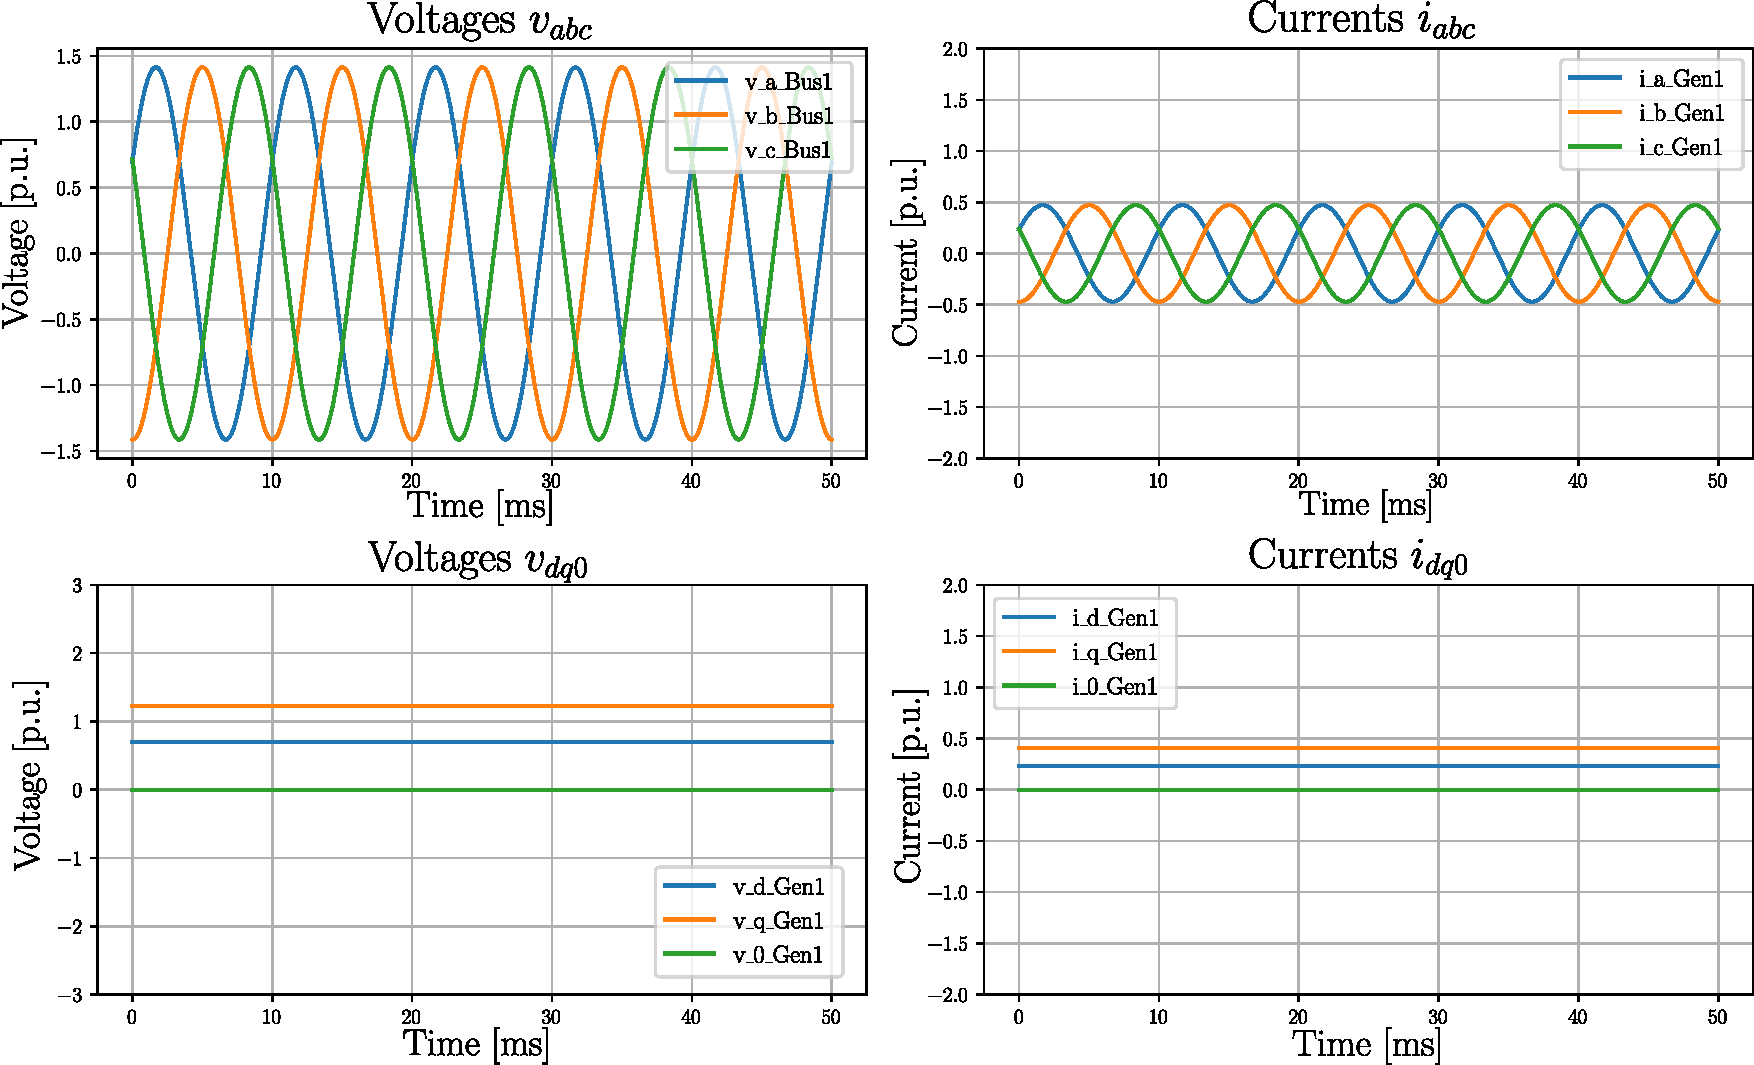
\includegraphics[width=1\linewidth]{figures/generator_load_1bus_rload3pu/voltages_currents.pdf}
    \caption{Voltages and currents at the 1 bus case.}
    \label{fig:voltages_currents_generator}
\end{figure}

Figures \ref{fig:theta_generator} and \ref{fig:omega_generator} show the rotor angle and angular speed of the generator rotor, respectively. 
The rotor angle $\theta$ increases linearly as expected due to the constant angular speed, while the angular speed $\omega$ remains at 1.0 p.u. 
during the whole simulation confirming steady state operation. The rotor is spinning at positive speed meaning it is delivering power to the load as expected.
This can also be seen at the angle graph, where the angle increases positively with time and in the voltages and currents graphs, where the order of the phases
is A-B-C, confirming positive direction of rotation.

\begin{figure}[htbp!]
    \centering
    \begin{minipage}[t]{0.48\textwidth}
        \centering
        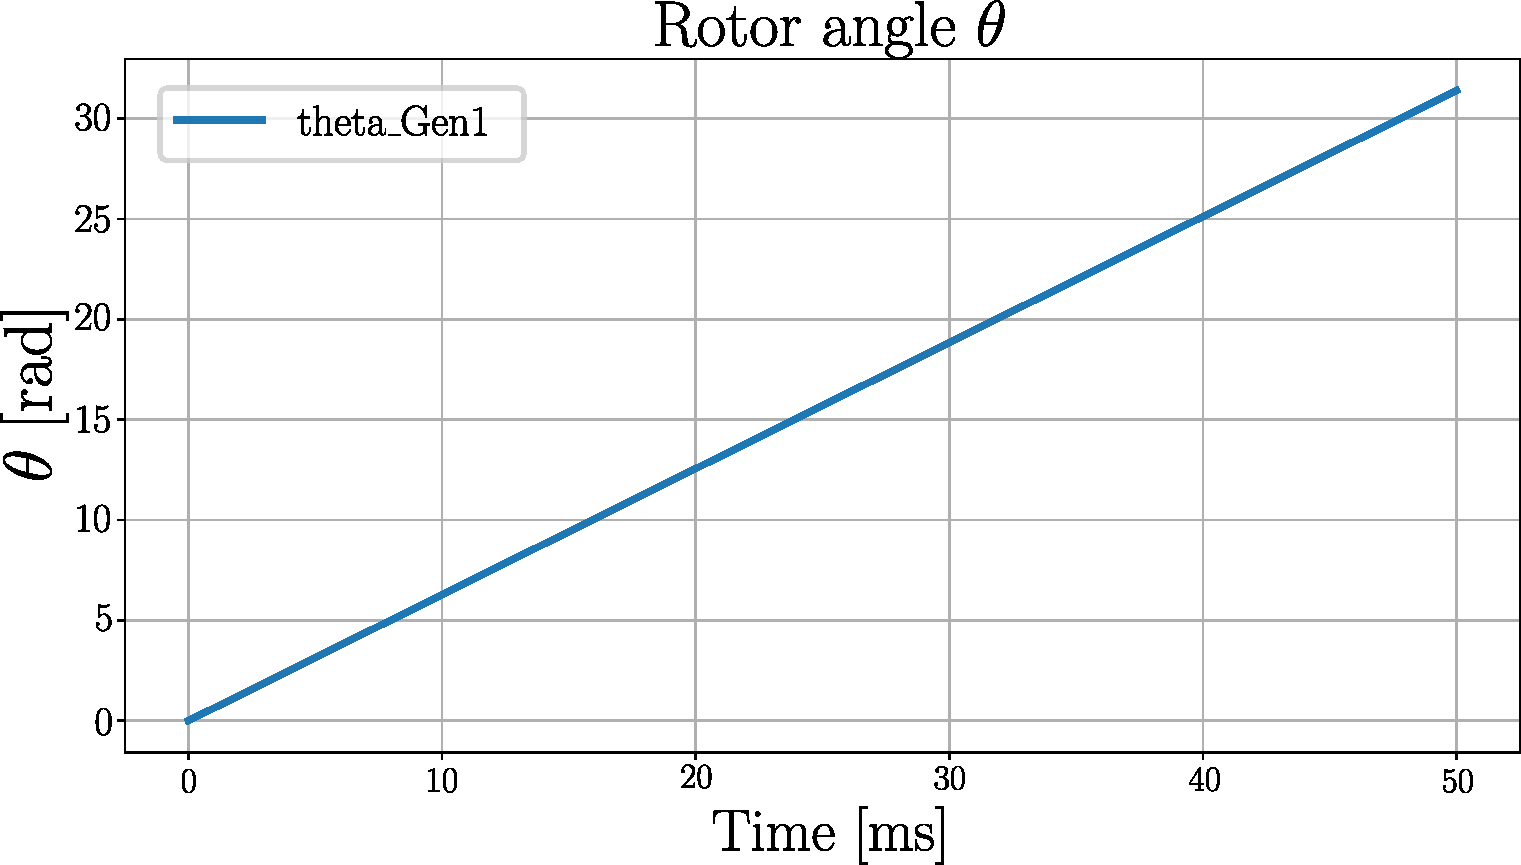
\includegraphics[width=\linewidth]{figures/generator_load_1bus_rload3pu/theta.pdf}
        \captionof{figure}{Rotor angle $\theta$ of the generator.}
        \label{fig:theta_generator}
    \end{minipage}\hfill
    \begin{minipage}[t]{0.48\textwidth}
        \centering
        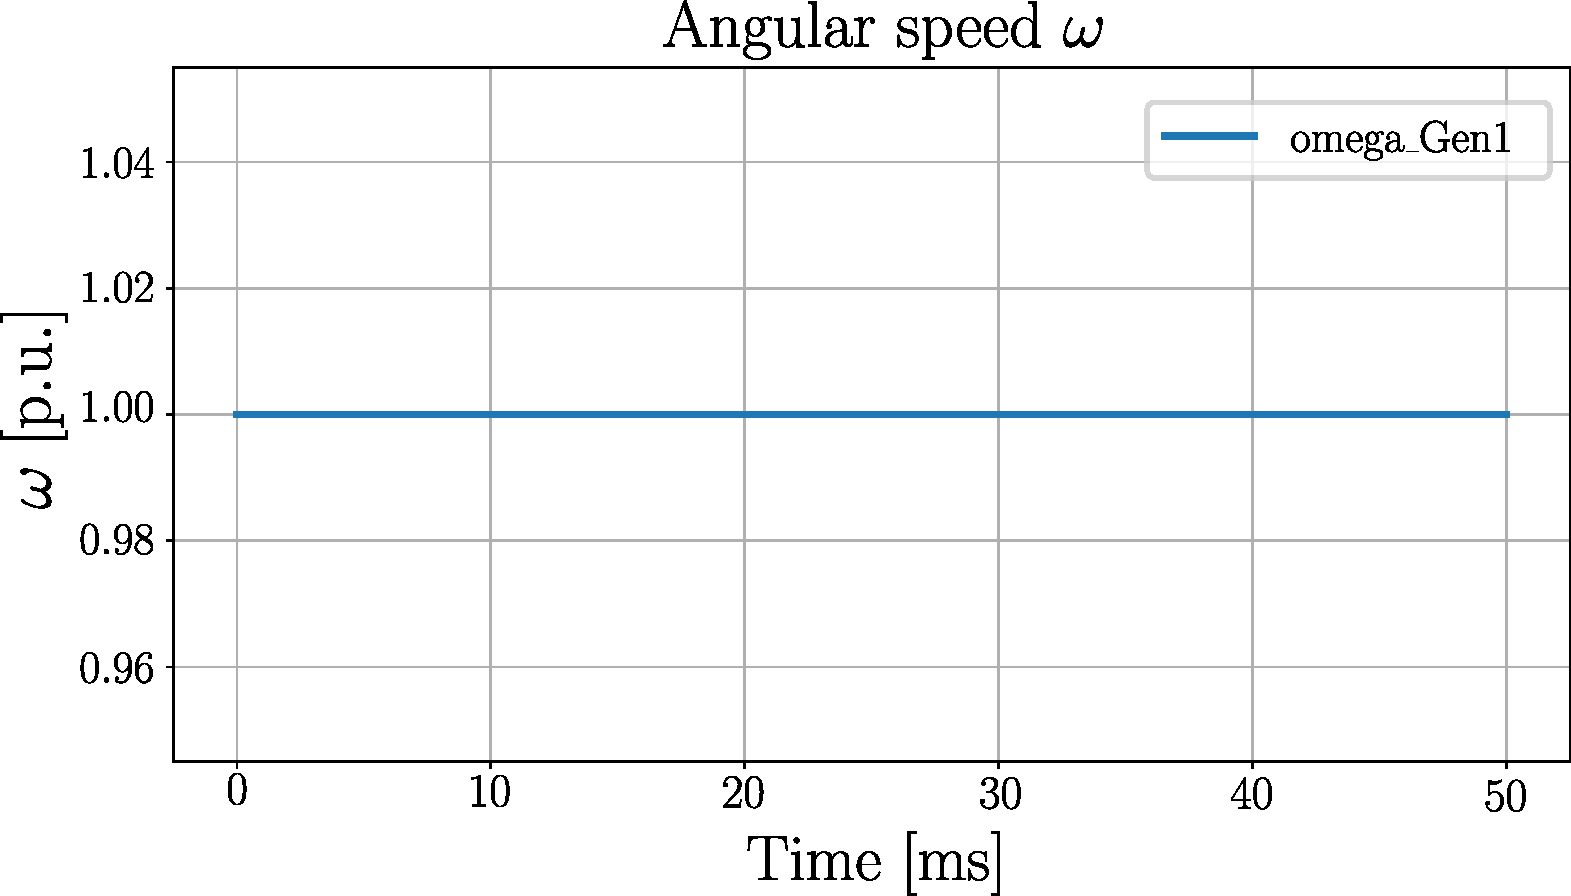
\includegraphics[width=\linewidth]{figures/generator_load_1bus_rload3pu/omega.pdf}
        \captionof{figure}{Angular speed $\omega$ of the generator rotor.}
        \label{fig:omega_generator}
    \end{minipage}
\end{figure}

Figures \ref{fig:torques_generator} and \ref{fig:powers_generator} show the electrical and mechanical torques and powers, respectively. 
The electrical torque $\Gamma_e$ and power $P_e$ remain constant during the simulation, and exactly equal to the mechanical torque $\Gamma_m$ and power $P_m$,
all of them at 1 p.u. confirming that the generator is operating at the nominal point. Since the model assumes no losses, the electrical and mechanical magnitudes coincide.
The reactive power is constant at 0.0 p.u. as expected due to the resistive load connected. Overall, the generator is correctly
supplying the load with the required power.

\begin{figure}[htbp!]
    \centering
    \begin{minipage}[t]{0.48\textwidth}
        \centering
        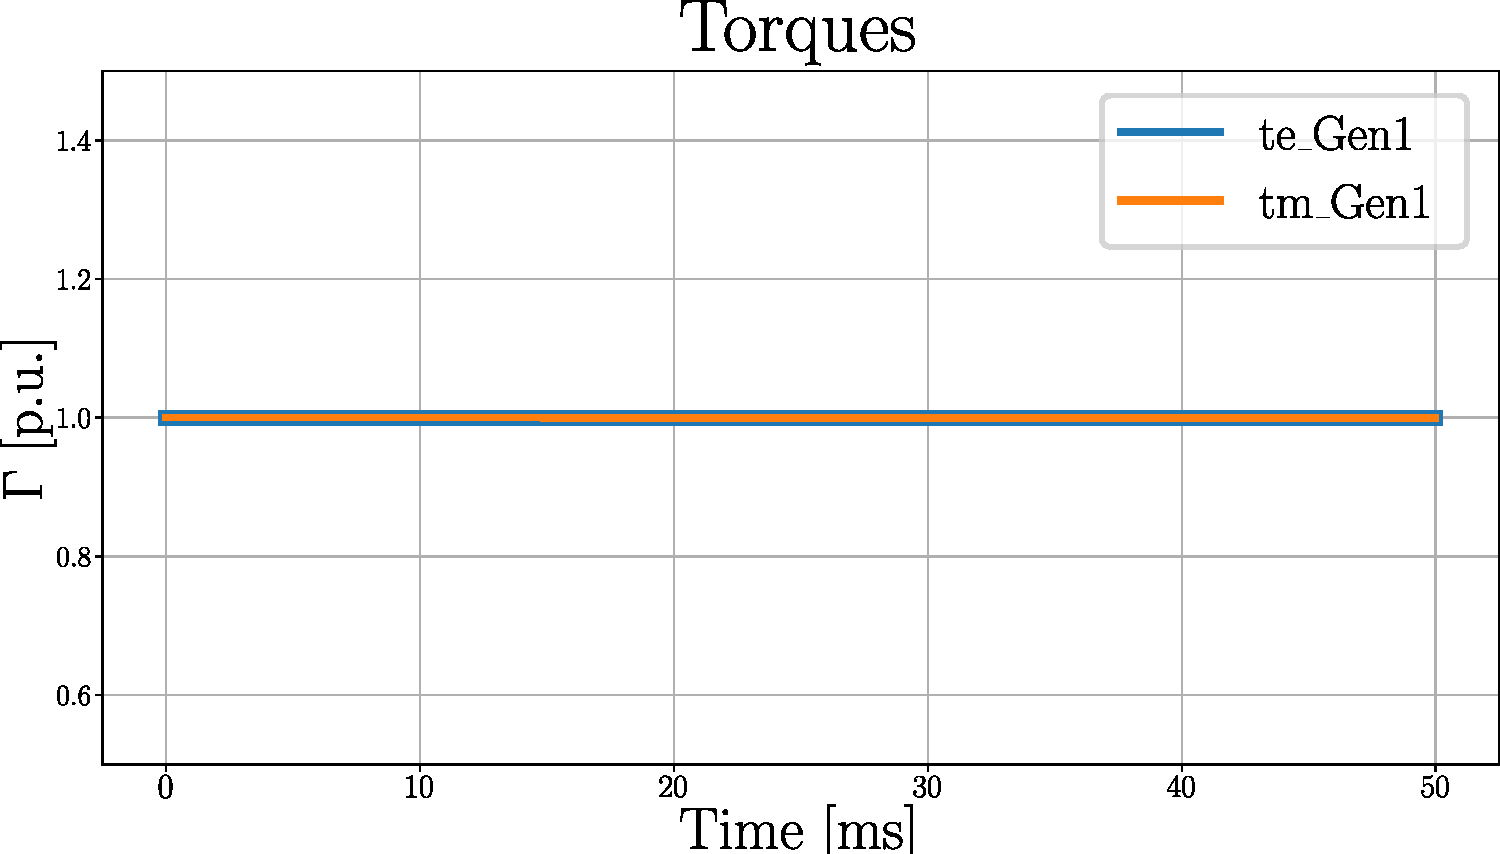
\includegraphics[width=\linewidth]{figures/generator_load_1bus_rload3pu/torques.pdf}
        \captionof{figure}{Electrical $\Gamma_e$ and mechanical $\Gamma_m$ torque of the generator.}
        \label{fig:torques_generator}
    \end{minipage}\hfill
    \begin{minipage}[t]{0.48\textwidth}
        \centering
        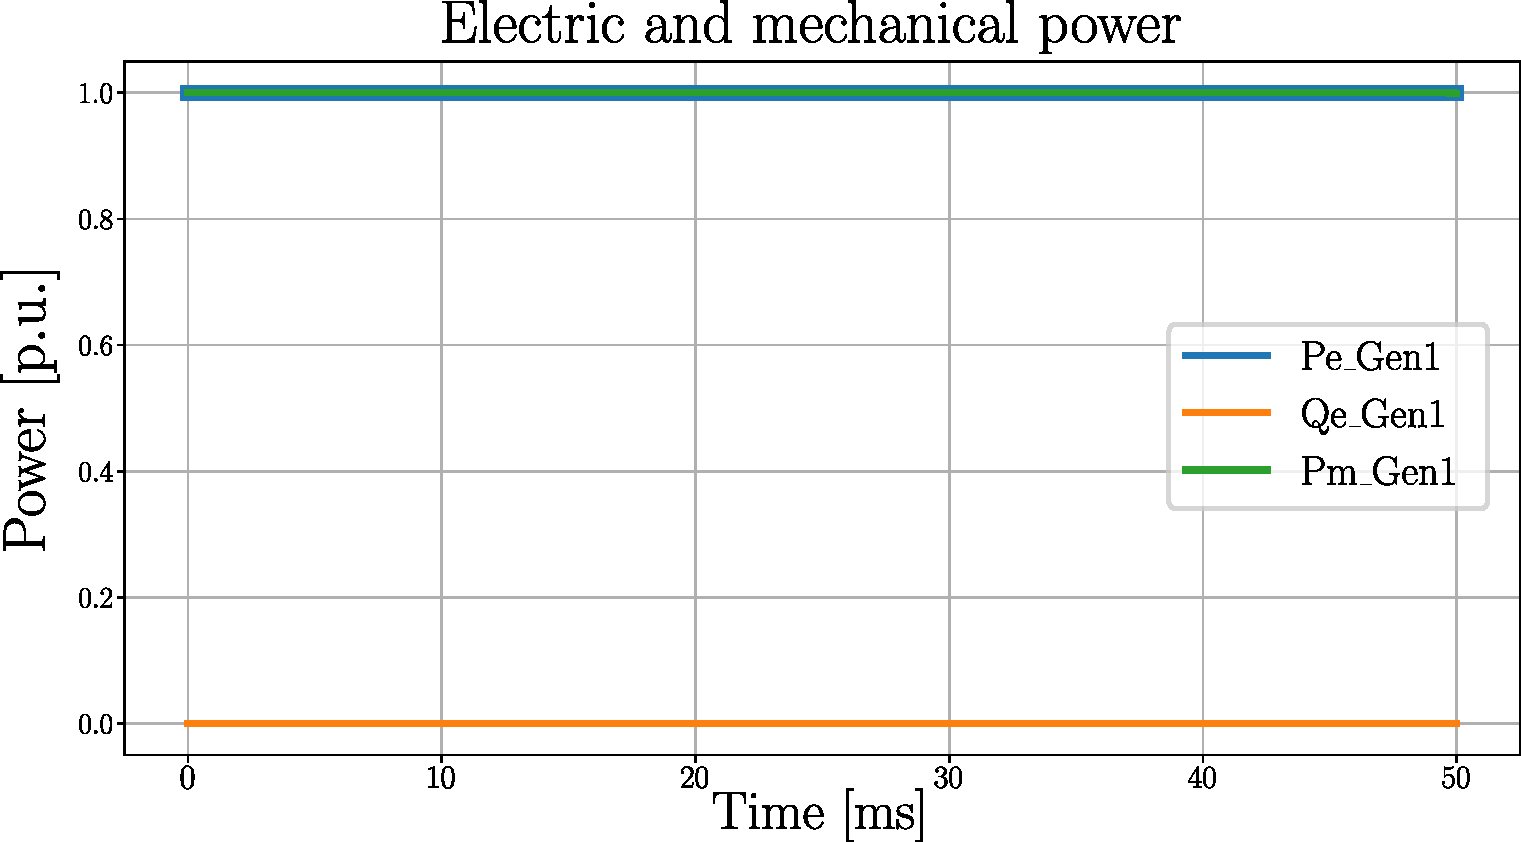
\includegraphics[width=\linewidth]{figures/generator_load_1bus_rload3pu/power.pdf}
        \captionof{figure}{Electrical $P_e$, $Q_e$ and mechanic power $P_m$ of the generator rotor.}
        \label{fig:powers_generator}
    \end{minipage}
\end{figure}

Finally, Figure \ref{fig:derivatives_generator} show the derivatives of the state variables of the generator. 
As seen, all derivatives remain at 0.0 confirming that the system is at steady state during the whole simulation. Only one derivative 
remains at $2\pi f$, which is the derivative of the rotor angle $\theta$, confirming that the rotor is spinning at nominal speed. 

\begin{figure}[h!]
    \centering
    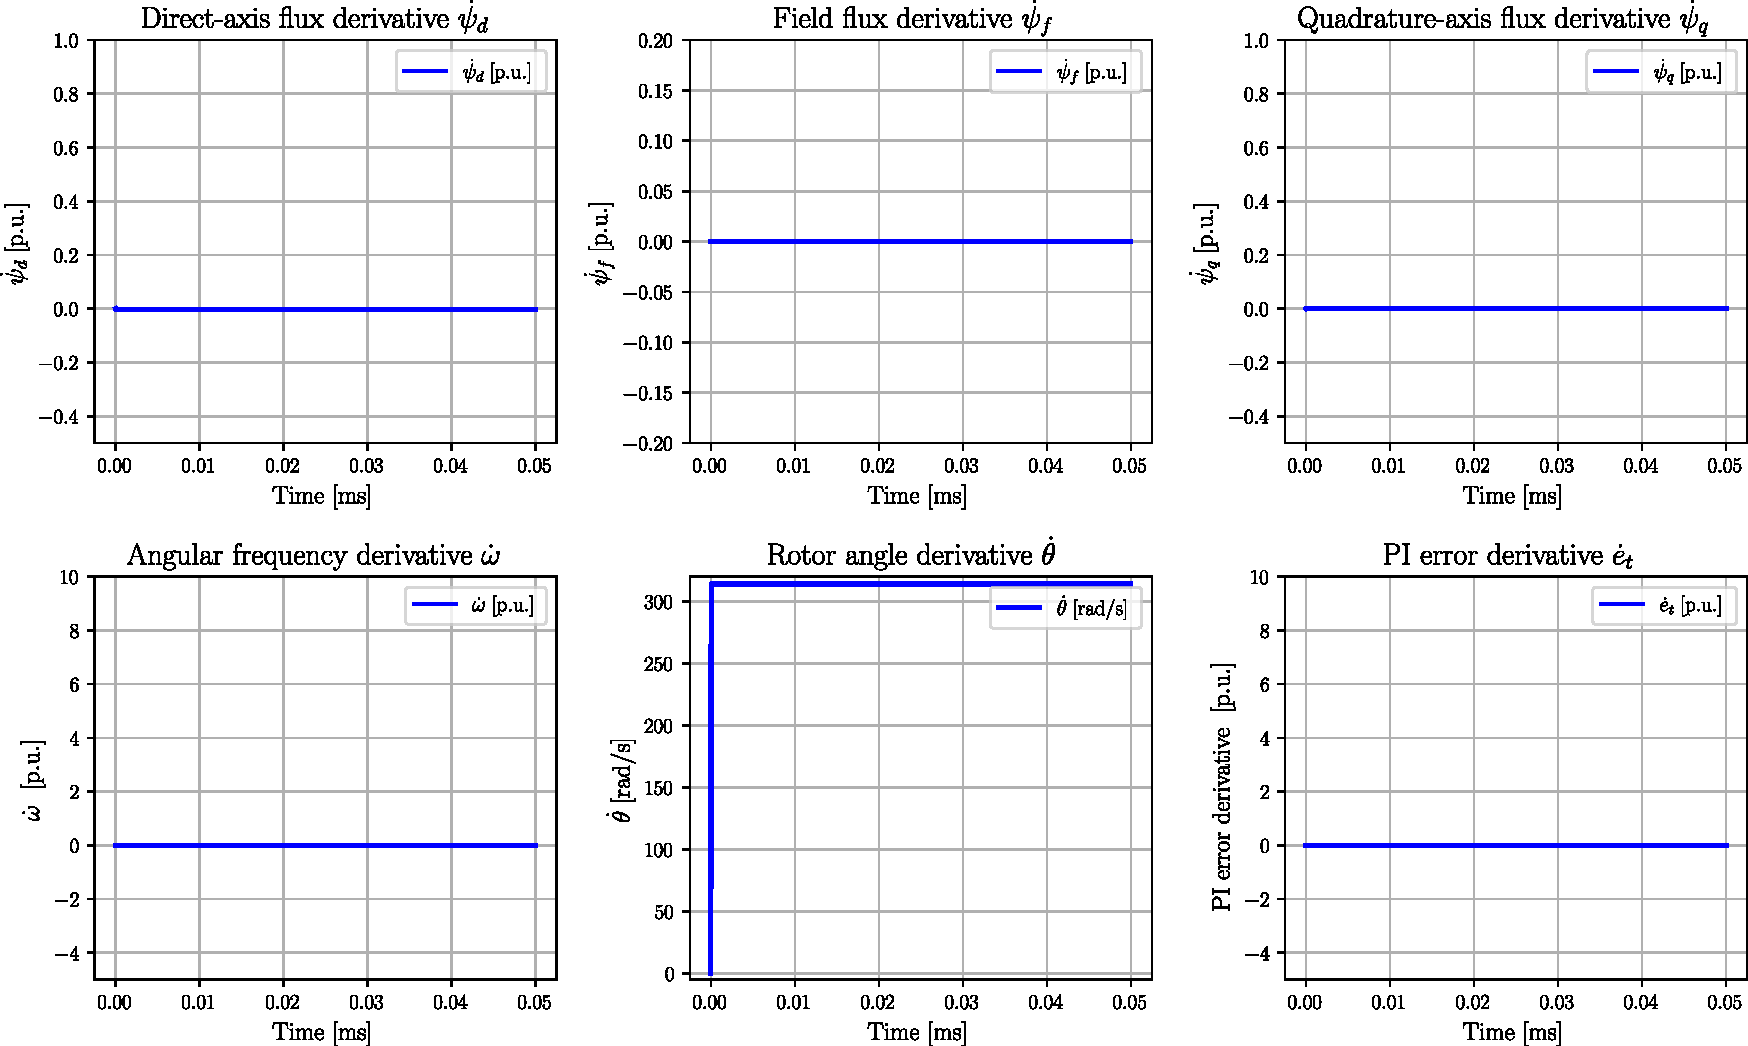
\includegraphics[width=1\linewidth]{figures/generator_load_1bus_rload3pu/derivatives.pdf}
    \caption{Derivatives of state variables at the 1 bus case.}
    \label{fig:derivatives_generator}
\end{figure}



\subsubsection{Test case 2: 2 bus case.}

This test case consists on a simple 2 bus system where a three-phase synchronous generator is connected to a three-phase load by means of a three-phase line.
This is the simplest test case possible considering a system (more than one bus) where the line model can be tested. The system diagram is shown in Figure \ref{fig:2bus_case_diagram}.
Three different scenarios are simulated to test the line model: matched $Z_c$ resistance, short-circuited receiving end and open-circuited receiving end. Table \ref{tab:test_case_2_parameters} 
summarizes the main parameters of the system.
\begin{table}[htbp]
\centering
\caption{Main parameters of the synchronous generator, transmission line, and load for the travelling-wave test cases.}
\label{tab:test_case_2_parameters}
\renewcommand{\arraystretch}{1.2}
\begin{tabular}{|l|l|c|l|}
\hline
\textbf{Parameter} & \textbf{Description} & \textbf{Magnitude} & \textbf{Units} \\
\hline
\multicolumn{4}{|l|}{\textbf{Synchronous generator}} \\
\hline
-- & Generator EMT-type model & Same as Test Case~1 & -- \\
\hline
\multicolumn{4}{|l|}{\textbf{Transmission line}} \\
\hline
Line name & Line identifier & Line 1--2 & -- \\
Length & Line physical length & 100 & km \\
Rated power & Thermal rating & 200 & MVA \\
Voltage level & Nominal line-to-line voltage & $V_\text{base}$ & kV \\
\hline
\multicolumn{4}{|l|}{\textit{Tower and conductor geometry}} \\
\hline
Tower type & Overhead line configuration & Tower & -- \\
Conductor type & Phase conductor & Panther 30/7 ACSR & -- \\
Outer diameter & Conductor external diameter & 21.0 & mm \\
Inner diameter & Conductor internal diameter & 9.0 & mm \\
DC resistance & Conductor resistance & 0.1363 & $\Omega$/km \\
Maximum current & Thermal current limit & 1.0 & p.u. \\
\hline
Phase A position & Horizontal / vertical position & $(-12.65,\;27.5)$ & m \\
Phase B position & Horizontal / vertical position & $(0,\;27.5)$ & m \\
Phase C position & Horizontal / vertical position & $(12.65,\;27.5)$ & m \\
\hline
\multicolumn{4}{|l|}{\textbf{Load / termination conditions}} \\
\hline
Case~1 & Matched termination & $Z_\text{load} = Z_c$ & p.u. \\
Case~2 & Short-circuit termination & $Z_\text{load} = 0$ & p.u. \\
Case~3 & Open-circuit termination & $Z_\text{load} \rightarrow \infty$ & -- \\
\hline
\end{tabular}
\end{table}



\begin{figure}[h!]
    \centering
    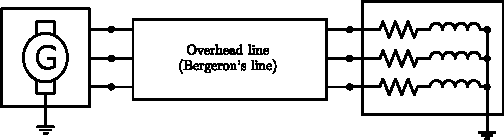
\includegraphics[width=0.8\linewidth]{inkscape_svg/line_test_eq_circuit.pdf}
    \caption{Test case 2: Two-bus system diagram.}
    \label{fig:2bus_case_diagram}
\end{figure}

\textbf{Matched $Z_c$ resistance.}

In this case, the impedance at the receiving end is set to match the characteristic impedance of the line.

The results shown in Figures~\ref{fig:matched_voltages} and~\ref{fig:matched_line_currents} show a clear time shift of exactly one propagation delay
$\tau$ between the waveforms measured at the sending and receiving ends of the line, both for
voltages and currents. This behavior is a direct consequence of the travelling-wave nature of
electromagnetic transients in distributed-parameter transmission lines, as described by the
telegrapher's equations. In this formulation, voltage and current disturbances propagate along
the line as forward and backward travelling waves at a finite velocity determined by the line
inductance and capacitance per unit length.

In this test case, the load is perfectly matched to the characteristic impedance of the line
($Z_{\text{load}} = Z_c$), which eliminates impedance discontinuities at the receiving end.
As a result, no reflected waves are generated, and all the incident energy is absorbed by the
load. Under these conditions, the voltage and current waveforms at the receiving end correspond
exactly to the incident waves delayed by the line travel time $\tau$, without distortion or
superposition with reflected components. The same reasoning applies at the sending end, where
the absence of reflections ensures that the source does not experience any delayed feedback
from the line.

This explains the identical waveform shapes observed at both ends of the line, with the only
difference being a pure time delay equal to the propagation time, which is the expected behaviour
of a lossless Bergeron-type line model under matched termination.


\begin{figure}[h!]
    \centering
    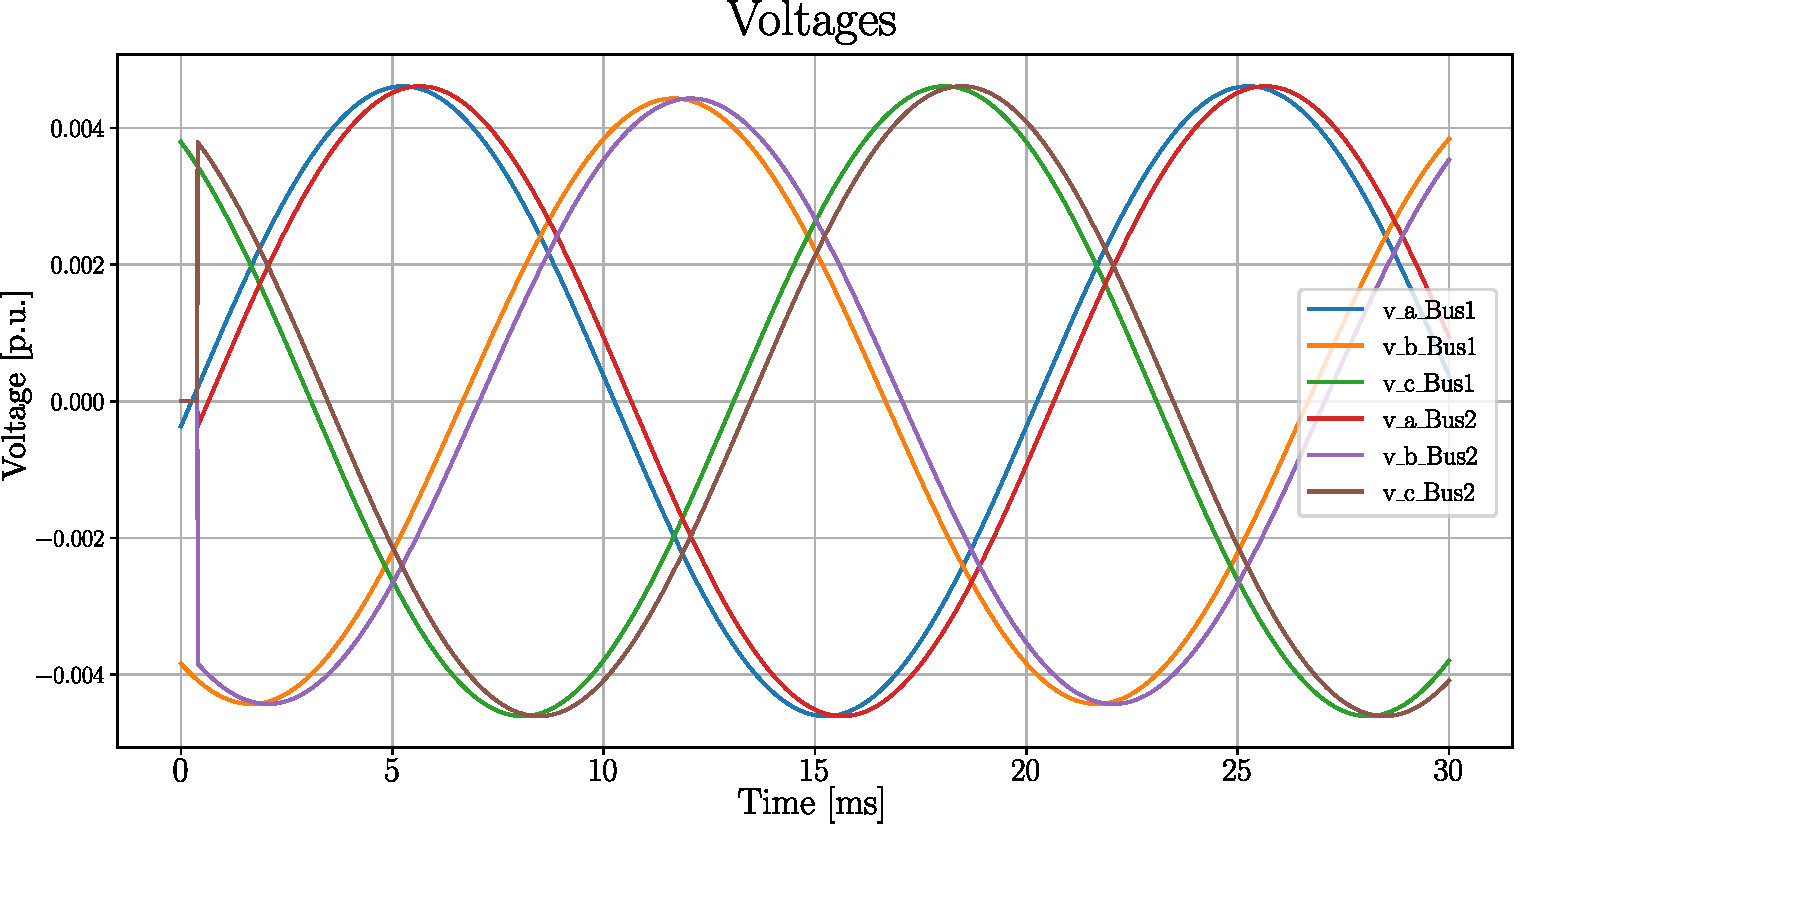
\includegraphics[width=0.8\linewidth]{figures/vsource_line_3ph/Voltages_matched.pdf}
    \caption{Voltages at the 2 bus case. WITH VOLTAGE SOURCE!! TO CHANGE}
    \label{fig:matched_voltages}
\end{figure}
\begin{figure}[h!]
    \centering
    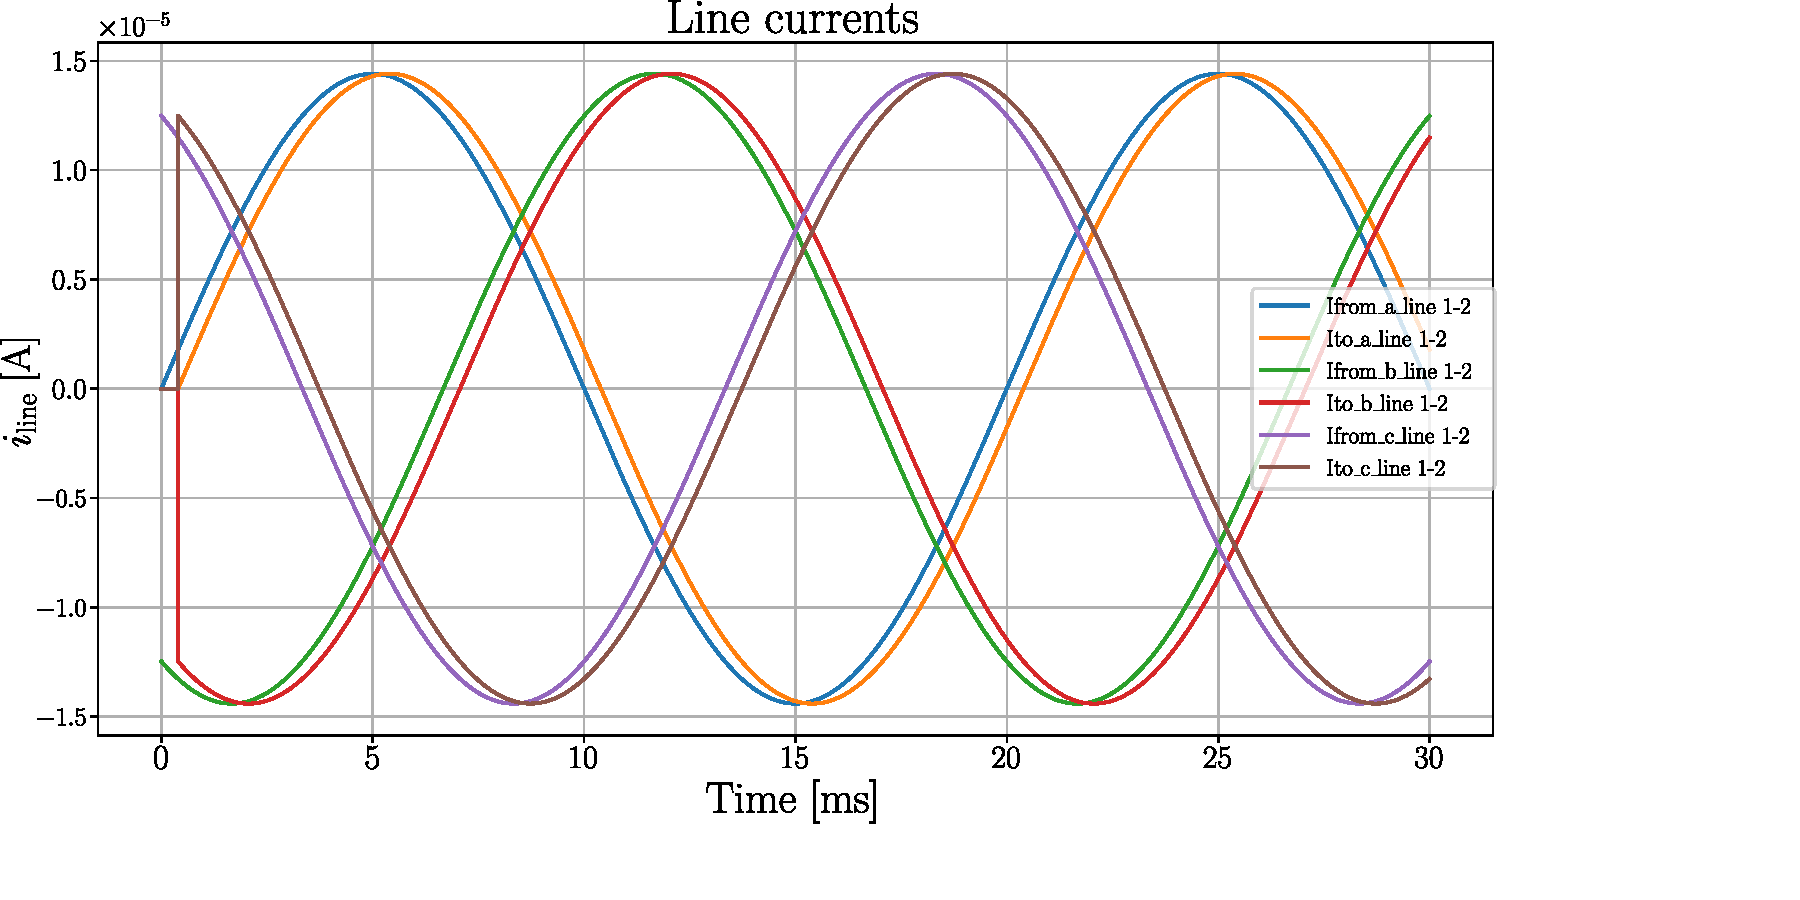
\includegraphics[width=0.8\linewidth]{figures/vsource_line_3ph/line_currents_matched.pdf}
    \caption{Line currents at the 2 bus case. WITH VOLTAGE SOURCE!! TO CHANGE}
    \label{fig:matched_line_currents}
\end{figure}

\textbf{Short-circuited receiving end.}

\begin{comment}
The results corresponding to the short-circuited receiving end show a markedly different
behavior compared to the matched-load case, while still exhibiting clear propagation
effects governed by the travelling-wave formulation. As in the previous case, voltage and
current disturbances propagate along the line according to the telegrapher's equations, with
a finite propagation time $\tau$ determined by the distributed inductance and capacitance of
the line. However, the short-circuit condition at the receiving end introduces a strong
impedance discontinuity that fundamentally alters the wave interaction.

For a short-circuited termination ($Z_{\text{load}} = 0$), the voltage reflection coefficient is
equal to $-1$, while the current reflection coefficient is $+1$. Consequently, when the
incident wave reaches the receiving end, the voltage wave is fully reflected with opposite
polarity, whereas the current wave is reflected with the same polarity. This results in a zero
voltage condition at the receiving end, as imposed by the short circuit, and a doubling of the
current amplitude due to the superposition of the incident and reflected current waves.

The reflected waves then propagate back towards the sending end, reaching it after an
additional delay $\tau$. As a result, the sending-end waveforms exhibit changes after a total
round-trip time of $2\tau$, reflecting the interaction between the source and the reflected
waves from the faulted termination. This process may lead to waveform distortion or
amplitude changes depending on the source impedance and boundary conditions at the
sending end.

Overall, the observed voltage and current waveforms are consistent with classical travelling-
wave theory for short-circuited lines: the presence of full reflections at the receiving end,
the inversion of voltage waves, the reinforcement of current waves, and the appearance of
delayed effects at the sending end after integer multiples of the line propagation time.
This behaviour confirms the correct representation of wave reflections and boundary
conditions in the Bergeron-type line model.


\begin{figure}[h!]
    \centering
    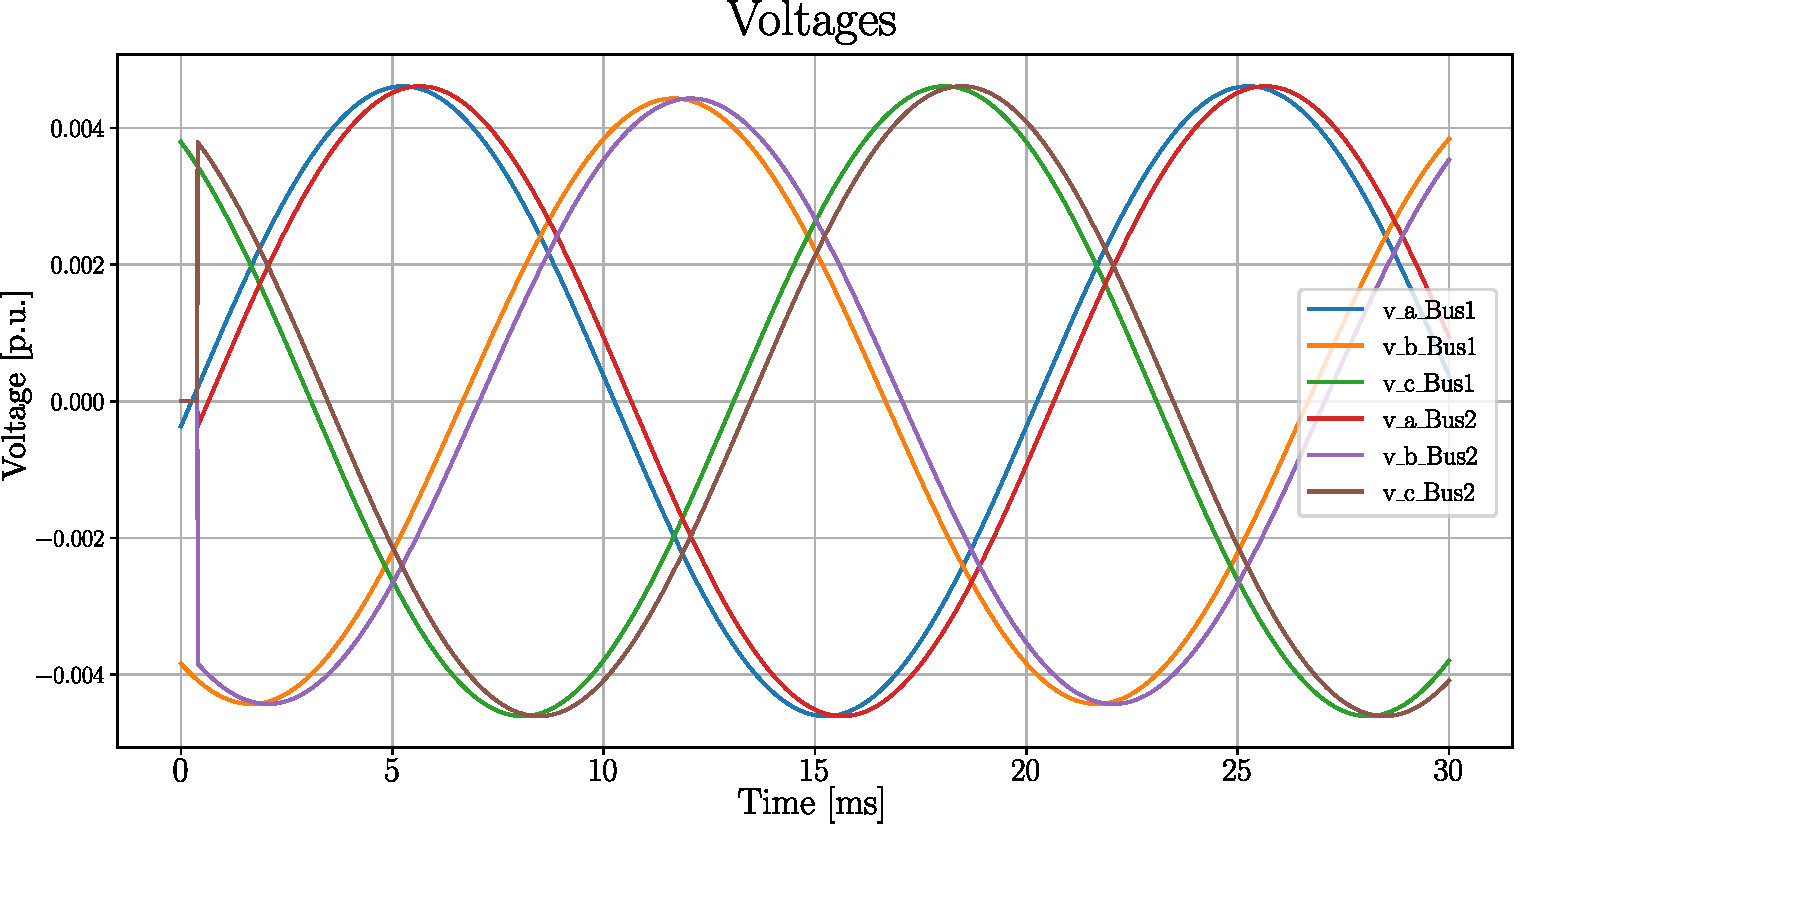
\includegraphics[width=0.8\linewidth]{figures/vsource_line_3ph/Voltages_matched.pdf}
    \caption{Voltages at the 2 bus case.}
    \label{fig:short_circuit_line_voltages}
\end{figure}
\begin{figure}[h!]
    \centering
    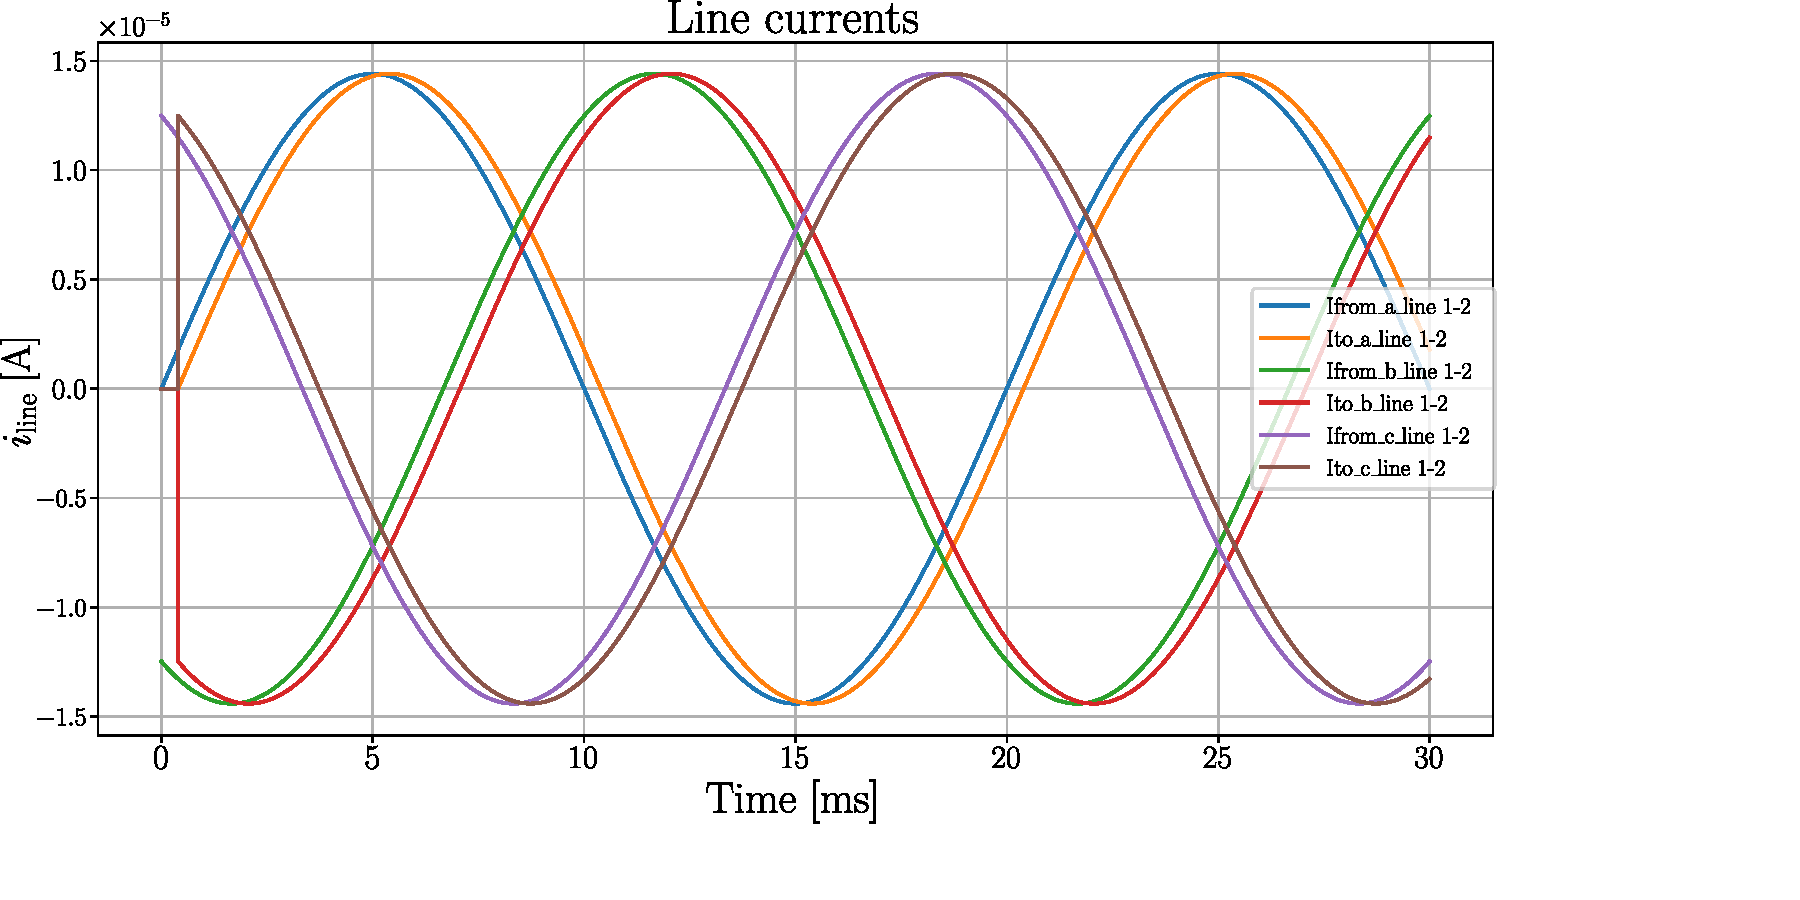
\includegraphics[width=0.8\linewidth]{figures/vsource_line_3ph/line_currents_matched.pdf}
    \caption{Line currents at the 2 bus case.}
    \label{fig:short_circuit_line_line_currents}
\end{figure}

\end{comment}

\textbf{Open-circuited receiving end.}

\begin{comment}

The results corresponding to the open-circuited receiving end again exhibit travelling-wave
behaviour governed by the telegrapher's equations, but with reflection characteristics that
differ from both the matched-load and short-circuit cases. Voltage and current disturbances
propagate along the line with a finite propagation time $\tau$, determined by the distributed
inductance and capacitance of the line, giving rise to delayed interactions between the
sending and receiving ends.

For an open-circuit termination ($Z_{\text{load}} \rightarrow \infty$), the voltage reflection
coefficient is equal to $+1$, while the current reflection coefficient is $-1$. When the
incident wave reaches the receiving end, the voltage wave is fully reflected with the same
polarity, whereas the current wave is reflected with opposite polarity. As a consequence, the
current at the receiving end is forced to zero, as imposed by the open-circuit condition,
while the voltage amplitude is doubled due to the superposition of the incident and reflected
voltage waves.

The reflected waves propagate back towards the sending end and reach it after an additional
delay $\tau$, so that changes in the sending-end waveforms appear after a total round-trip
time of $2\tau$. These delayed effects reflect the interaction between the source and the
reflections generated at the open termination, and may result in transient overvoltages or
waveform distortion depending on the source impedance.

Overall, the observed waveforms are fully consistent with classical travelling-wave theory
for open-circuited lines: complete reflection of voltage waves without polarity inversion,
complete reflection of current waves with polarity inversion, zero current at the receiving
end, and delayed feedback at the sending end after multiples of the propagation time. This
confirms the correct modelling of boundary conditions and wave reflections in the Bergeron-
type transmission line representation.


\begin{figure}[h!]
    \centering
    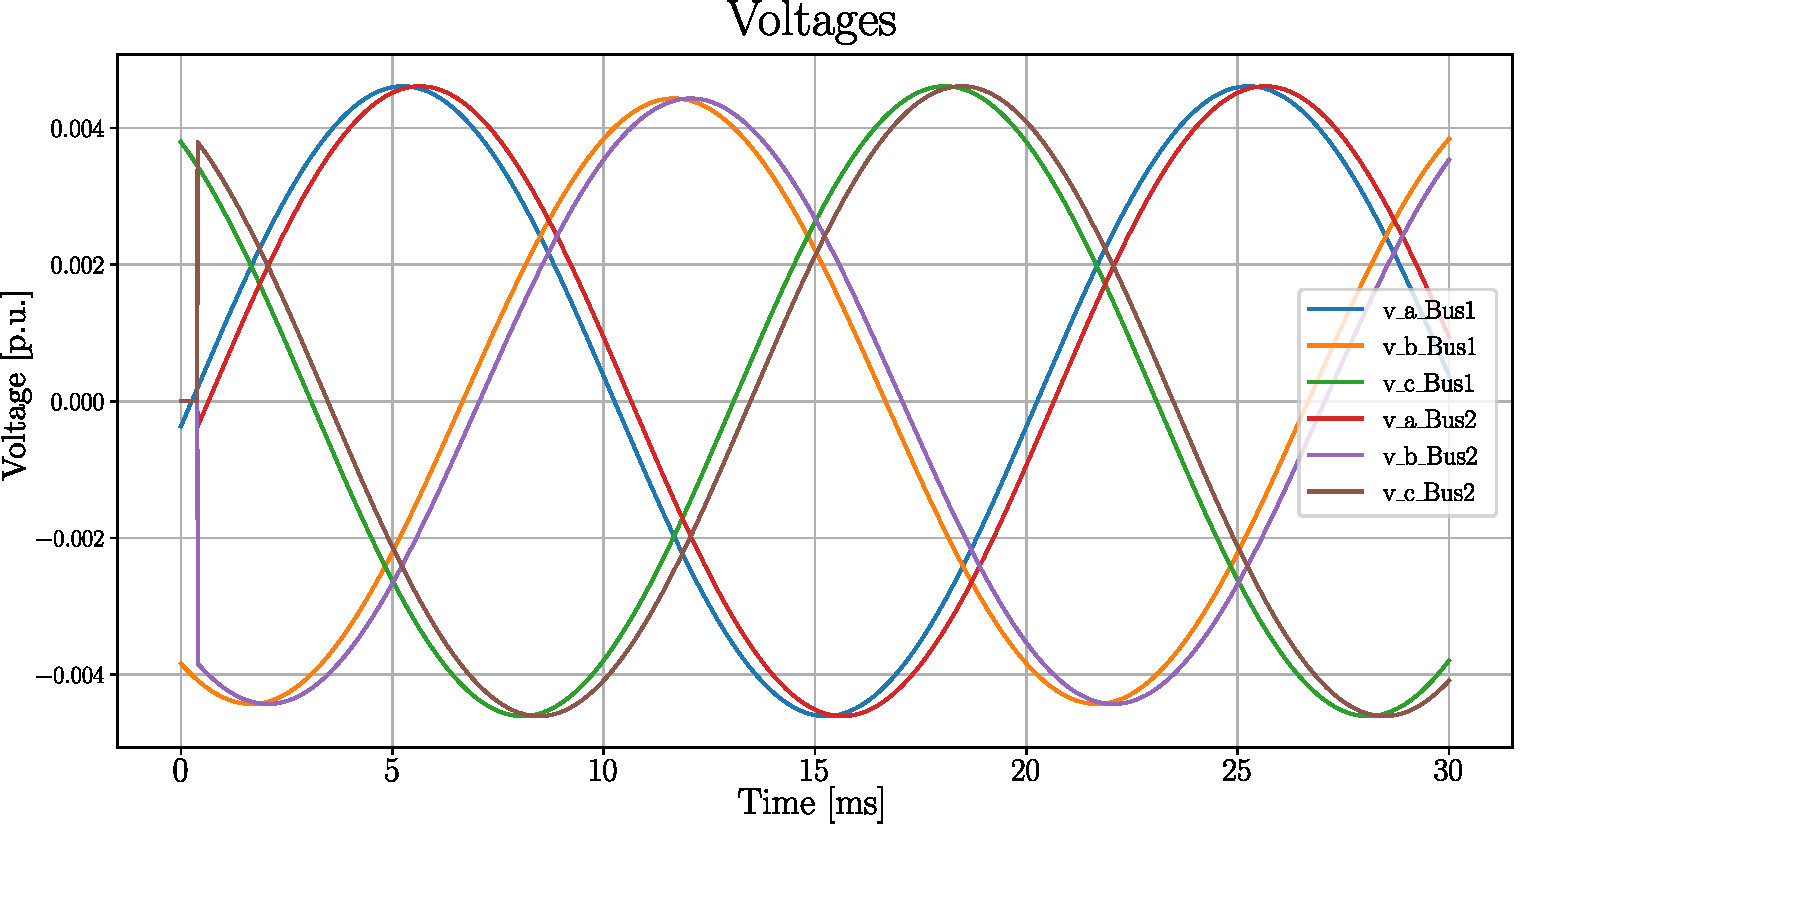
\includegraphics[width=0.8\linewidth]{figures/vsource_line_3ph/Voltages_matched.pdf}
    \caption{Voltages at the 2 bus case.}
    \label{fig:open_circuit_line_voltages}
\end{figure}
\begin{figure}[h!]
    \centering
    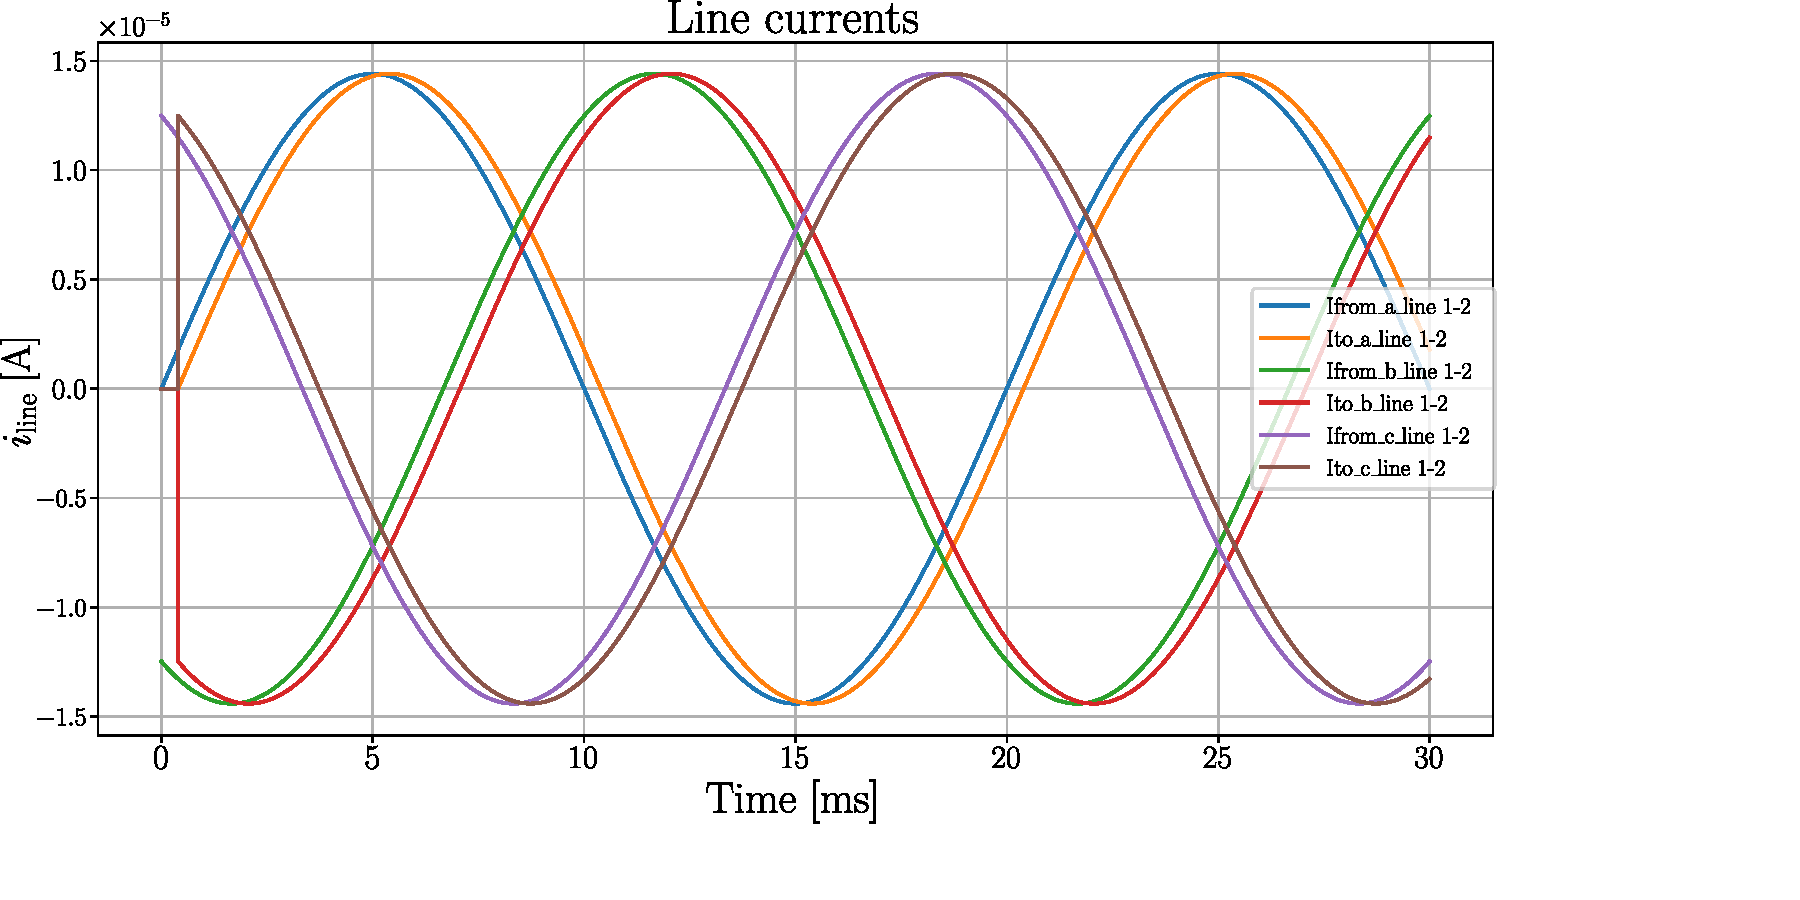
\includegraphics[width=0.8\linewidth]{figures/vsource_line_3ph/line_currents_matched.pdf}
    \caption{Line currents at the 2 bus case.}
    \label{fig:open_circuit_line_line_currents}
\end{figure}
\end{comment}